\documentclass[12pt,a4paper]{article}
\usepackage[utf8]{inputenc}
\usepackage{amsmath}
\usepackage{amsfonts}
\usepackage{amssymb}
\usepackage{graphicx}
\usepackage{subcaption}
\usepackage[top=2in, bottom=1.5in, left=1in, right=1in]{geometry}
\usepackage{fancyhdr}
\pagestyle{fancy}
\fancyhf{}
\rhead{Hunter King B00528551\\Alex Rudiuk B00672069}
\author{Hunter King and Alex Rudiuk}
\title{CSCI 6505 Assignment $\#$7}
\begin{document}
\section*{CSCI 6505 Assignment $\#$7}
\subsection*{Intro}
This assignment explores and compares reinforcement learning through the use of a static \textbf{look-up table??} and a function approximator as a means to learn to play tic-tac-toe and ``four in a row". Initially the system was trained against itself using the Q-learning algorithm as a means of training. Once the system was trained, a second system composed of a function approximator that used a sigmoidal multilayer perceptron was also trained. This second system used the same Q-learning algorithm to update the weights of the function approximator, but also used a back propagation method to update the weights once each game was completed.\\
It should be noted to give context to the results that if an individual knows how to play tic-tac-toe well they should never lose due to a rather limited number of ways to play. This then extends such that if two players who both know how to play play against each other, the result will always be a tie. This also extends to ``four-in-a-row"
\subsection*{Methods}
\subsubsection*{Q-learning Tic-Tac-Toe}
The first method used for tic-tac-toe was the Q-learning algorithm utilizing a lookup table. The lookup table stores the value of every potential board state. These values were stored in a 9 dimensional array such that the system can quickly point to an index and retrieve the corresponding value of the state instead of searching through a list for the state in question. though this method requires a significant amount of memory, it also allows for a significant increase in training (and testing) speed. The lookup table was initialized with random values ranging from $[-0.5 \rightarrow 0.5]$. Once the system was initialized, it was trained by playing against itself for 3 million games, updating the table through the Q-learning method (equation \ref{eq:q-learning}). 
\begin{equation}
{Q(s,a)} \leftarrow {Q(s,a) + \mu(r + \gamma max_{a'}Q(s',a')-Q(s,a))}
\label{eq:q-learning}
\end{equation}
The results of the training are shown in figure \ref{fig:training}
\begin{figure}[h]
\centering
\begin{subfigure}[h]{0.45\textwidth}
\includegraphics[width=\textwidth]{Figures/train01epsilon.png}
\end{subfigure}
\begin{subfigure}[h]{0.45\textwidth}
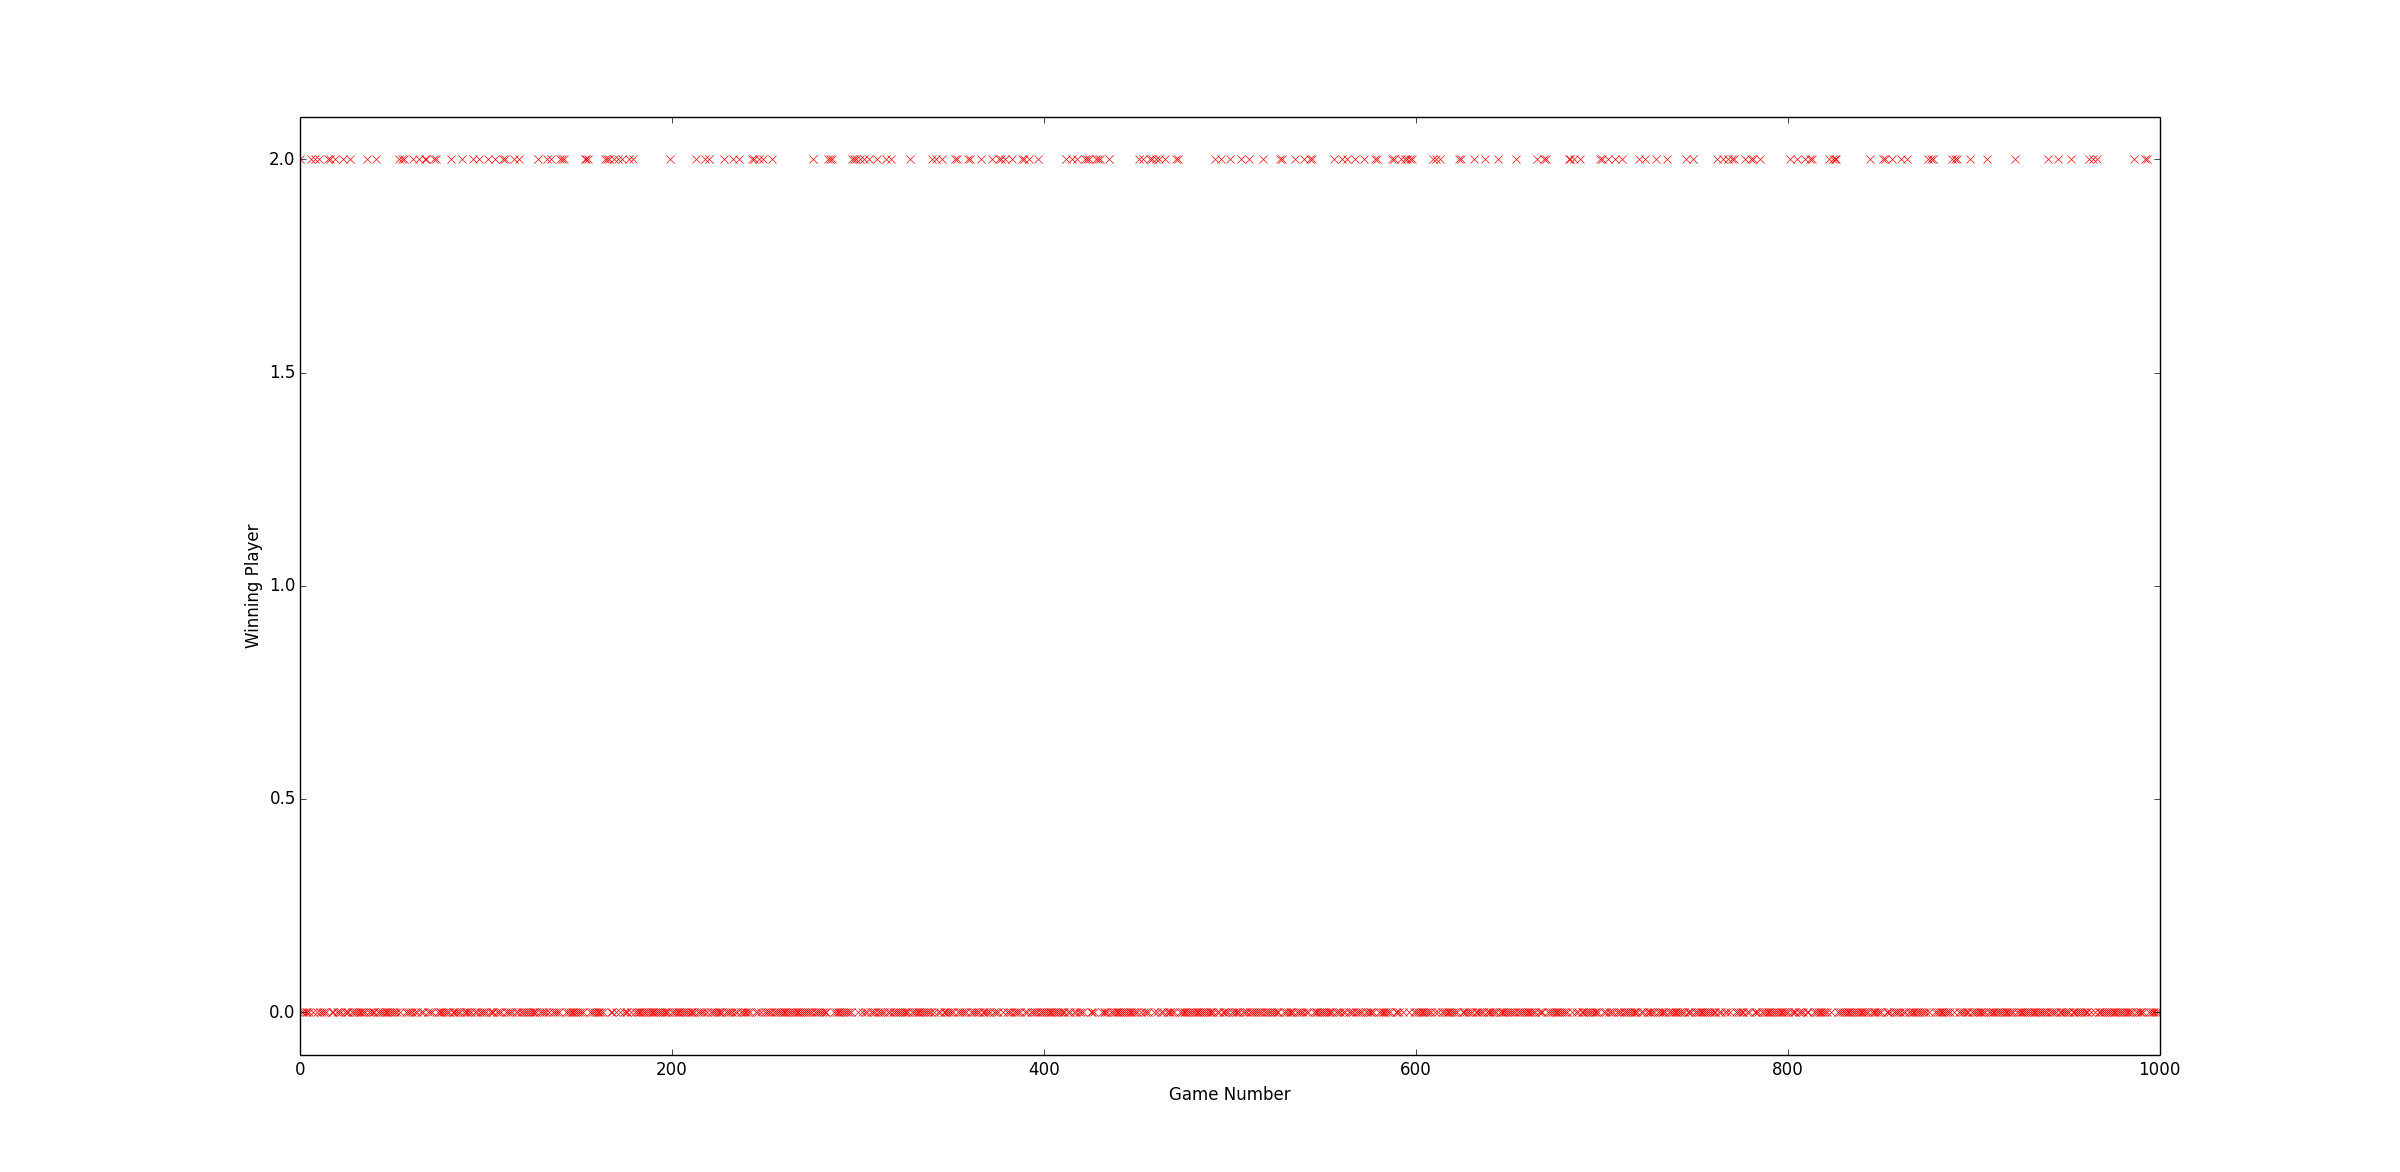
\includegraphics[width=\textwidth]{Figures/Optimalstateresults.png}
\end{subfigure}
\caption{Left: Average results over training period, bins are 10000 games. Right: Trained system playing against a trained system with 10\% chance to make random move.}
\label{fig:training}
\end{figure}
The plot shows an average of $\sim$32\% wins. Meaning that 32/100 games end in not a tie. This imperfect result is due to our $\epsilon$ (random action selection) which we set to 0.1. Figure BB show the results of the same trained system, but with $\epsilon$=0, playing against a version of itself with $\epsilon$=0.1.
The output is 2.0 whenever the player with $\epsilon$=0 wins, and is 1.0 when the player with $\epsilon$=0.1 wins. This proves that our system has learned to properly play the game as both players mostly tie, however due to the 10\% chance of a random move by the opponent, the player sometimes wins (though never loses).
\subsection*{Q-learning Four-in-a-row}
Although Q-learning worked very well for tic-tac-toe, it unfortunately did not scale very well. Using Q-learning for tic-tac-toe with a lookup table required $3^{9}$ states to be stored, and due to the nature of the method used, this was stored 3 times over. This equated to a requirement of 4MB of memory to store. When this is scaled up to the $3^{16}$ positions required for the four-in-a-row game it required ~24GB of memory. We unfortunately did not have access to a computer with that amount of RAM so we could not complete the game with our lookup table algorithm.
\subsubsection*{Function approximator}
A solution to the problem of poor scaling (the ``curse of dimensionality") is to use a function approximator to replace the lookup table. This function approximator uses a multilayer perceptron with a single hidden layer. The inputs correspond to the board state and the selected action (move). This requires only 28 inputs for tic-tac-toe and 49 inputs for four-in-a-row (see figure \ref{fig:funcApproxFigure}). The inputs are composed of 3 inputs for each potential position on the board and 1 final input for the action (move) to be made. The three board location input correspond to either player one in location (100), player 2 in location (010), or no player in location (001).
\begin{figure}[h]
\centering
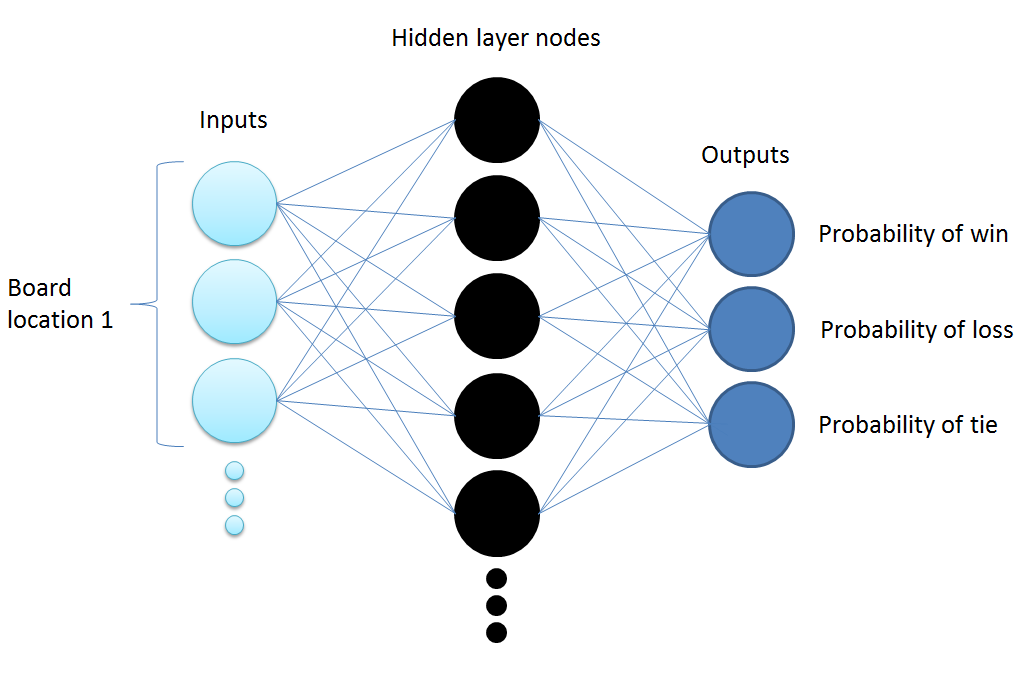
\includegraphics[width=0.8\textwidth]{Figures/functionApproxFigure.png}
\caption{Multilayer perceptron used as function approximator}
\label{fig:funcApproxFigure}
\end{figure}
Memory usage is significantly reduced with a function approximator compared to a lookup table. A function approximator only needs to store the weights between nodes, inputs, and ouputs. Therefore, for tic-tac-toe with 40 hidden nodes used (40 was the optimal number of nodes selected by Gerald Tesauro for use in TD learning for backgammon), the system would only need to store 1240 weights. This is a significant reduction from the $\sim$19000 states stored by the lookup table. The function approximator scales $O(n)$, where the lookup table scales $O(3^{n})$. However, the function approximator is not better in every way than the lookup table. Since the lookup table stores the specific value of a board state, and the function approximator works as it sounds (approximates this function), it is not fair to expect a perfectly trained system however the results were... \textbf{INSERT SECTION ON RESULTS HERE}.
\pagebreak
\subsection*{Conclusions}

\end{document}